\chapter{實驗設計及結果討論}
\label{chapter:experiment}

本研究的主要貢獻為基準商品資料集、物品夾取可行性評估、以及主動式操作系統。為了評估這3個貢獻,本研究透過此資料集的訓練資料集進行訓練,並使用測試集執行任務與評估品牌文字切割的準確度。本實驗預期透過以下實驗評估1. 透過本資料集(一個場景只出現單個物體)所訓練的品牌文字語意切割模型在複雜場景(遮蔽、重疊),也就是本研究設計的測試集,表現效果如何。2. 透過基於品牌文字與物品語意之夾取可行性視覺系統的主動式機器人操作系統,對於特定姿態放置的任務的表現效果如何,本部分將重現測試集的場景,並在同樣場景中用不同方法進行任務,已進行比較。

\section{實驗一、品牌文字切割評估}
本研究利用現實世界測試集評估具旋轉差異性的品牌文字切割,評量的單位有以圖片為單位以及以品牌文字為單位的。換句話說,會針對單張圖片每一個畫素所預測出的品牌文字標註與人為標註(groundtruth)比較,也會對測試集的所有場景中出現過的品牌文字標註(groundtruth),與預測結果比較。

\subsection{分類模型的評估方法介紹}

\paragraph{F-score}
在語意切割模型評估指標方法中,常使用到精確率(Precision)與召回率(Recall),精確率定義$\frac{TP}{TP + FP}$。代表分類為真實正確的樣本數,占所有被分類為正確的樣本數的比例。,而召回率定義為$\frac{TP}{TP + FN}$,代表分類為正確的樣本數,占應該被分為正類的比例。兩者在大型資料庫中,分數往往是會有制約的狀況。換句話說,當模型的精確率高時,召回率便會較低。反之亦然。而F-score則是權衡兩個評估方式,所產生了一個新的計算公式:。這個方法被大量用於像素級別的類別預測的評估方法。

\paragraph{Intersection of Union (IOU)}
Intersection over Union是物件偵測模型評估指標方法中,經常被使用到的方法,定義為$\frac{Prediction \cap  Groundtruth}{Prediction \cup  Groundtruth}$,也就是在預測結果與真實結果的聯集中,預測結果與真實結果交集的比率。通常數值大於0.5便可稱之為不錯。FCN ~\cite{long2015fully}也是使用此方法進行語意切割模型的評估。

\subsection{實驗設計}



本研究設計了表格~\ref{tbl:segmentation},縱軸為資料庫的所有子測試集,用來測試品牌文字切割模型,並以雜亂、遮蔽情況為標準,由簡單到複雜往下排列,橫軸則為評量的標準,第一部分為以場景(圖片)為單位的評估。這部分以F-score評估模型對整體圖片品牌文字切割的準確度。而第二部分則以所有場景中的所有品牌文字為單位,如此設計的原因是夾取可行性評估是以單一品牌文字預測標註遮罩與姿態作為線索,因此本研究十分重視對於每一個品牌文字語意切割預測的表現結果。在表格中有提供每一個子資料集所出現的可視的品牌文字數量、以及每個品牌文字預期結果與人為标注結果(groundtruth)的比較,並以IOU進行評量。依照人感官而言,IOU大於50\%,已經是很好的結果,看起來十分接近,因此本實驗預期整理出IOU大於50\%比例,並基於品牌文字皆為單行,可用旋轉矩形框住比擬的假設,針對這些品牌文字切割遮罩以一個旋轉矩形框住,去分析預測結果與真實標註的$\Delta\theta$((~\ref{figure:iou_deltatheta}))。

\subsection{實驗結果與討論}
雖然在~\cite{zeng2016multi}的文獻中提出用單一物品於單一場景的訓練資料進行訓練,能在多物品複雜的場景中有好的成效,但參考表格中F-score一欄,可發現物體愈多,愈嚴重的雜亂情況下,會造成逐漸降低的F-score。同樣的以品牌文字為單位的評估中,雜亂環境也會增加預測出低IOU($ \le$ 0.5)的比率,以及惡化預測出高IOU($ \ge$  0.5)的品牌文字$\Delta\Theta$的大小,這些都會影響之後的主動式操作系統。

\subsection{失敗案例分析}
本研究觀察單一品牌文字偵測IOU$ \le$ 0.5之失敗案例,共將常出現之失敗案例分為四類。第一類(a)為不完整的遮罩。不完整的遮罩容易會造成之後,無論位置或是文字方向,品牌姿態預測的誤差。第二類(b)為類別的誤判,在此部分,不僅雖然品牌文字的部分有被偵測,但卻預測錯類別,會導致之後夾取與放置的方式錯誤,造成夾取失敗或是放錯格子的問題。第3類(c)為角度的誤判。一張圖片會以4個不同旋轉角度旋轉後再預測,最後整合為同一張圖片。此類的誤判是在錯誤的角度誤判到品牌文字,雖然偵測到品牌文字,也有正確的類別,卻會造成品牌文字方向的預測失敗。第4類(d)在商品的其餘部分偵測出品牌文字。這一類情況容易發生於較為雜亂的環境中。

\begin{figure}[ht]
	\centering
	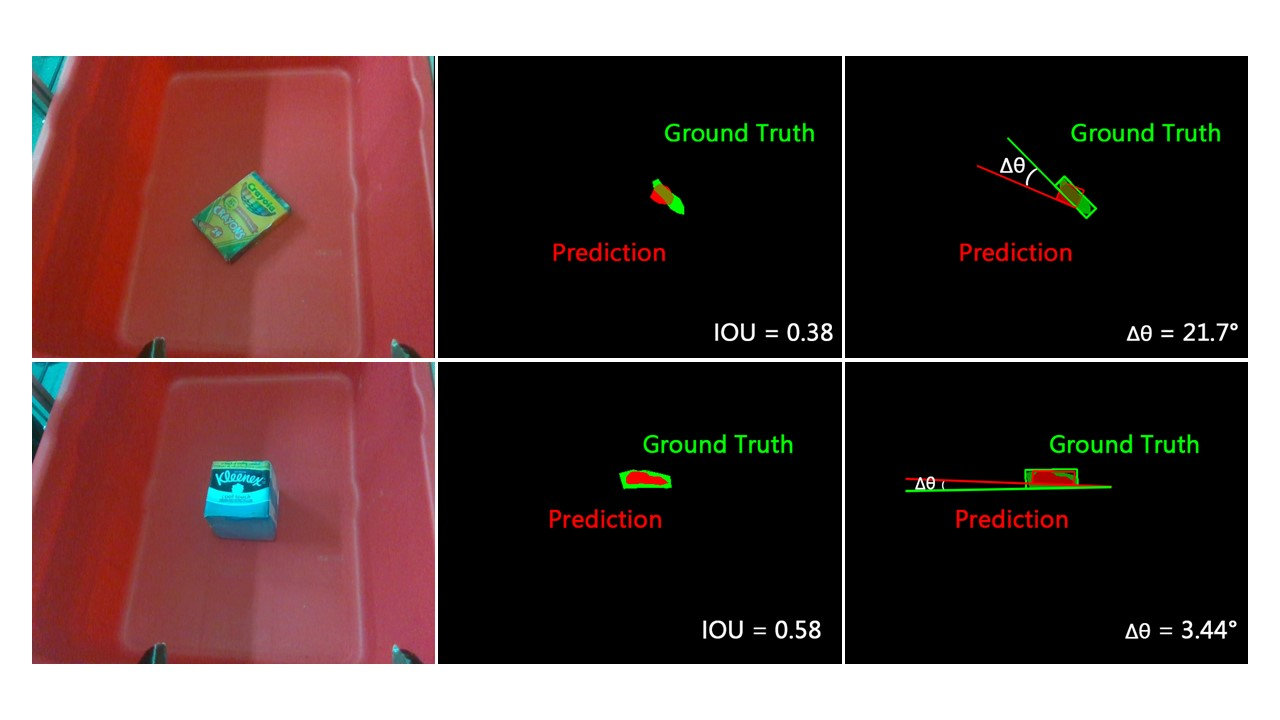
\includegraphics[height=!, width=0.8\linewidth, keepaspectratio=true]
	{./figures/iou_deltatheta.jpg}
  \caption{品牌文字語意切割的IoU與$\delta\theta$範例。低IoU與會造成較大的$\delta\theta$,並可能直接影響夾取可行性系統,造成之後的主動式操作系統夾取失敗。反之亦然,IoU愈高,則$\delta\theta$愈小,夾取可行性預測將愈準確。}
  \label{figure:iou_deltatheta}
\end{figure}

\begin{table}[tb]
\centering
\caption{品牌文字語意切割模型評估表. Scene: 場景的數量, Vis. BN: 可是品牌文字的數量, Num.: 品牌文字IoU 小於 0.5的數量。}
\label{tbl:segmentation}
\tabcolsep=4pt
\begin{tabular}{l|cc|crcc}
\hline
                               & \multicolumn{2}{c|}{Image-level}                         & \multicolumn{4}{c}{Brandname-level}                                                                                        \\ \hline
\multirow{2}{*}{Benchmark}     & \multirow{2}{*}{Scene}    & \multirow{2}{*}{F-score}     & \multirow{2}{*}{Vis. BN}     & \multicolumn{1}{|c|}{IoU $<$ 0.5} & \multicolumn{2}{c}{IoU $\ge$ 0.5}                                  \\ \cline{5-7}
                               &                           &                              &                         & \multicolumn{1}{|c|}{Num. (\%)}        & \multicolumn{1}{c|}{Ave. IoU} & \multicolumn{1}{c}{$\Delta$$\theta$} \\ \hline
Single-1                       & 50                        & 0.70                & 50                      & 7  (14\%)                         & 0.72                          &  5.45                               \\
Duplicated-2                   & 90                        & 0.66                         & 145                     & 32 (22\%)                         & 0.71                          &  5.91                               \\
Multiple-2                     & 90                        & 0.66                         & 159                     & 36 (23\%)                         & 0.70                          &  5.64                               \\
Clutter-3                      & 20                        & 0.62                         & 31                      & 7  (23\%)                         & 0.73                          &  7.14                               \\
Clutter-5                      & 20                        & 0.60                         & 32                      & 11 (34\%)                         & 0.66                          &  7.77                               \\
Clutter-7                      & 20                        & 0.53                         & 59                      & 17 (29\%)                         & 0.70                          &  7.90                               \\ \hline
\end{tabular}
\end{table}

\begin{figure}[ht]
	\centering
	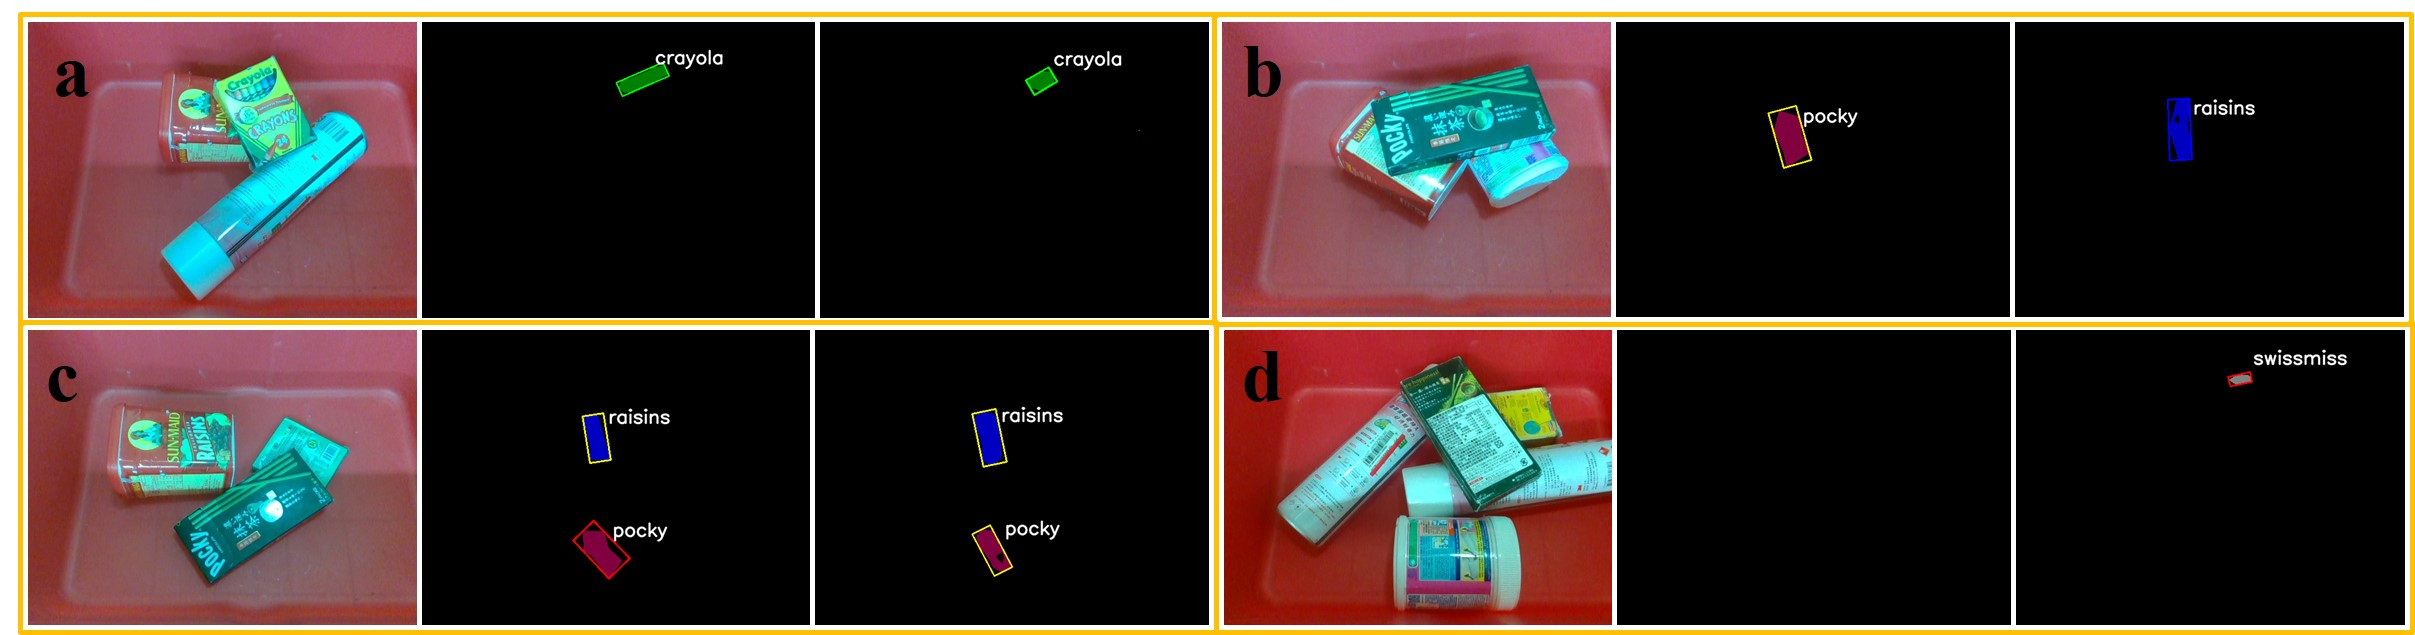
\includegraphics[height=!, width=0.8\linewidth, keepaspectratio=true]
	{./figures/failure_case.jpg}
  \caption{語意切割模型失敗範例。以品牌文字為單元,並以IoU = 0.5為門檻,定義小於0.5者為失敗的語意切割。本圖中共介紹4類常出現的失敗案例。}
  \label{figure:failure_case}
\end{figure}
